\documentclass{lab_sheet}
\usepackage{hyperref}
\usepackage{nccmath}
\newcommand\ddfrac[2]{\frac{\displaystyle #1}{\displaystyle #2}}


\newcommand{\proteusObservationA}[4]{ 
\begin{figure}[H]
   \begin{minipage}[b]{0.60\linewidth}
     \centering
     \includegraphics[width=\linewidth]{../Figures/#1.PDF}
   \end{minipage}%
   \begin{minipage}[b]{0.40\linewidth}
     \centering
 \begin{tabular}[b]{|M{4cm}|M{1cm}|}
   \hline
   \multicolumn{2}{|c|}{Noted Values} \\
   \hline \hline
   DC gain (in dB) & #2\\ \hline
   Half power frequency (in KHz) & #3\\ \hline
 \end{tabular}
 \end{minipage}
 \caption{Observation for #4}
 \label{fig:prot_obs_a_#1}
 \end{figure}
}


\newcommand{\proteusObservationB}[6]{ 
\begin{figure}[H]
   \begin{minipage}[b]{0.60\linewidth}
     \centering
     \includegraphics[width=\linewidth]{../Figures/#1.PDF}
   \end{minipage}%
   \begin{minipage}[b]{0.40\linewidth}
     \centering
 \begin{tabular}[b]{|M{4cm}|M{1cm}|}
   \hline
   \multicolumn{2}{|c|}{Noted Values} \\
   \hline \hline
   Gain in pass band (in dB) & #2\\ \hline
   Center frequency (in KHz) & #3\\ \hline
   Half power frequencies (in KHz) & #4\\ \hline
   Bandwidth (in KHz) & #5\\ \hline
 \end{tabular}
 \end{minipage}
 \caption{Observation for #6}
 \label{fig:prot_obs_b_#2}
 \end{figure}
}

\newcommand{\proteusObservationC}[4]{ 
\begin{figure}[H]
   \begin{minipage}[b]{0.60\linewidth}
     \centering
     \includegraphics[width=\linewidth]{../Figures/#1.PDF}
   \end{minipage}%
   \begin{minipage}[b]{0.40\linewidth}
     \centering
 \begin{tabular}[b]{|M{4cm}|M{1cm}|}
   \hline
   \multicolumn{2}{|c|}{Noted Values} \\
   \hline \hline
   Gain in pass band (in dB) & #2\\ \hline
   Half power frequency (in KHz) & #3\\ \hline
 \end{tabular}
 \end{minipage}
 \caption{Observation for #4}
 \label{fig:prot_obs_c_#2}
 \end{figure}
}

\newcommand{\proteusObservationD}[3]{ 
\begin{figure}[H]
   \begin{minipage}[b]{0.60\linewidth}
     \centering
     \includegraphics[width=\linewidth]{../Figures/#1.PDF}
   \end{minipage}%
   \begin{minipage}[b]{0.40\linewidth}
     \centering
 \begin{tabular}[b]{|M{4cm}|M{1cm}|}
   \hline
   \multicolumn{2}{|c|}{Noted Values} \\
   \hline \hline
    Gain in pass band (in $\mu$dB) & #2\\
    \hline
 \end{tabular}
 \end{minipage}
 \caption{Observation for #3}
 \label{fig:prot_obs_d_#2}
 \end{figure}
}

\newcommand{\figquestion}{
    \begin{circuitikz}[american]
        \draw
    (0,0) node [op amp] (opamp1) {}
    (4,-0.5) node [op amp] (opamp2) {}
    (8,-1) node [op amp] (opamp3) {}
  
    (-4,0.5) node [left] {$V_1$} to [R, l=$R_3$, o-*] (opamp1.-) |- (-0.75,2.25) to[short,*-*] (-1.2,2.25)
    (-0.75,3) to [R,l=$R_1$] (0.75,3) to (0.75, 1.5) to [C,l_=$C_1$] (-0.75, 1.5) to [short] (-0.75,3)
    (0.75,2.25) to[short,*-] (1.2,2.25) -| (opamp1.out) to [R, *-*,l=$R_4$] (opamp2.-) |- (2.8, 1.5) to[C,l=$C_2$] (5.2, 1.5) -| (opamp2.out) to [R, *-*,l=$R_5$] (opamp3.-)|- (6.8, 1.5) to[R,l=$R_5$,-*] (9.2, 1.5) -| (opamp3.out) |- (9.2,4.5) to [R, l_=$R_2$] (-1.2,4.5) -| (opamp1.-)
    
    (opamp1.+) node[ground] {}
    (opamp1.out) node[right,below] {$V_{O1}$}
    (opamp2.+) node[ground] {}
    (opamp2.out) node[right,below] {$V_{O2}$}
    (opamp3.+) node[ground] {}

    (9.8,-1) node [right] {$V_2$} to [short,o-*] (opamp3.out)
           ;
        \end{circuitikz}
}


\newcommand{\figbsap}{
    \begin{circuitikz}[american]
        \draw
    (0,0) node [op amp] (opamp1) {}
    (4,-0.5) node [op amp] (opamp2) {}
    (8,-1) node [op amp] (opamp3) {}
    (4,-6) node [op amp] (opamp4) {}
    
    (-4,0.5) node [left] {$V_1$} to [R, l=$R_3$, o-*] (opamp1.-) |- (-0.75,2.25) to[short,*-*] (-1.2,2.25)
    (-0.75,3) to [R,l=$R_1$] (0.75,3) to (0.75, 1.5) to [C,l_=$C_1$] (-0.75, 1.5) to [short] (-0.75,3)
    (0.75,2.25) to[short,*-] (1.2,2.25) -| (opamp1.out) to [R, *-*,l=$R_4$] (opamp2.-) |- (2.8, 1.5) to[C,l=$C_2$] (5.2, 1.5) -| (opamp2.out) to [R, *-*,l=$R_5$] (opamp3.-)|- (6.8, 1.5) to[R,l=$R_5$,-*] (9.2, 1.5) -| (opamp3.out) |- (9.2,4.5) to [R, l_=$R_2$] (-1.2,4.5) -| (opamp1.-)
    (opamp1.+) node[ground] {}
    (opamp1.out) node[inner sep=3pt,anchor=north west] {$V_{O1}$}
    (opamp2.+) node[ground] {}
    (opamp2.out) node[below] {$V_{O2}$}
    (opamp3.+) node[ground] {}
    (opamp4.+) node[ground] {}
    (9.8,-1) node [right] {$V_2$} to [short,o-*] (opamp3.out)
    (opamp1.out)|- (0,-1) to [short]
    (0,-5) to [R, l=$R_6$] (2,-5) to [short] (2,-6)
    to [R, l_=$R_6$] (0,-6)  to [short] (-3.5,-6) to [short,-*] (-3.5,0.5)
    (2,-5.5) to [short,*-*] (opamp4.-) |- (3,-4.5) to [R,l=$R_6$] (5,-4.5)-| (opamp4.out) to [short,*-o] (6,-6) node [right] {$V_{2}'$}
           ;
        \end{circuitikz}
}

\newcommand{\fighp}{
    \begin{circuitikz}[american]
        \draw
    (0,0) node [op amp] (opamp1) {}
    (4,-0.5) node [op amp] (opamp2) {}
    (8,-1) node [op amp] (opamp3) {}
    (4,-6) node [op amp] (opamp4) {}
    
    (-4,0.5) node [left] {$V_1$} to [R, l=$R_3$, o-*] (opamp1.-) |- (-0.75,2.25) to[short,*-*] (-1.2,2.25)
    (-0.75,3) to [R,l=$R_1$] (0.75,3) to (0.75, 1.5) to [C,l_=$C_1$] (-0.75, 1.5) to [short] (-0.75,3)
    (0.75,2.25) to[short,*-] (1.2,2.25) -| (opamp1.out) to [R, *-*,l=$R_4$] (opamp2.-) |- (2.8, 1.5) to[C,l=$C_2$] (5.2, 1.5) -| (opamp2.out) to [R, *-*,l=$R_5$] (opamp3.-)|- (6.8, 1.5) to[R,l=$R_5$,-*] (9.2, 1.5) -| (opamp3.out) |- (9.2,4.5) to [R, l_=$R_2$] (-1.2,4.5) -| (opamp1.-)
    (opamp1.+) node[ground] {}
    (opamp1.out) node[inner sep=3pt,anchor=north west] {$V_{O1}$}
    (opamp2.+) node[ground] {}
    (opamp2.out) node[below] {$V_{O2}$}
    (opamp3.+) node[ground] {}
    (opamp4.+) node[ground] {}
    (9.8,-1) node [right] {$V_2$} to [short,o-*] (opamp3.out)
    (opamp1.out)|- (0,-1) to [short]
    (0,-5) to [R, l=$R_6$] (2,-5) to [short] (2,-6)
    to [R, l_=$R_6$] (0,-6)  to [short] (-3.5,-6) to [short,-*] (-3.5,0.5)
    (2,-5.5) to [short,*-*] (opamp4.-) |- (3,-4.5) to [R,l=$R_6$] (5,-4.5)-| (opamp4.out) to [short,*-o] (6,-6) node [right] {$V_{2}'$}
    (opamp3.out)|-(9.2,-3.5) to [short] (5,-3.5) to [R,l_=$R_6$] (3,-3.5) to [short] (2.8,-3.5) to [short,-*] (2.8,-4.5)
           ;
        \end{circuitikz}
}

\newcommand{\figsecI}{
    \begin{circuitikz}[american]
\coordinate (A) at (1,3.75);
\coordinate (B) at (-1,3.75);
\coordinate (C) at (-1,1.25);
\coordinate (D) at (1,1.25);
\draw [dashed]  (A) to (B) to (C) to (D) to (A)
(0,3.75) node [above] {$Z=R_1//C_1$}
;
    \draw
    (0,0) node [op amp] (opamp) {}
    (-4,1) node [left] {$V_2$} to [R, l=$R_2$, o-] (-2,1) to [short] (-2,0)
    to [R, l_=$R_3$, -o] (-4,0) node [left] {$V_1$}
    (-2,0.5) to [short,*-*] (opamp.-) |- (-0.75,2.25) to[short,*-] (-1.2,2.25)
    (-0.75,3) to [R,l=$R_1$] (0.75,3) to (0.75, 1.75) to [C,l_=$C_1$] (-0.75, 1.75) to [short] (-0.75,3)
    (0.75,2.25) to[short,*-] (1.2,2.25) -| (opamp.out) to [short,*-o] (2,0) node [right] {$V_{O1}$}
    (opamp.+) node[ground] {}
    ;
        \end{circuitikz}
}

\newcommand{\figsecII}{
    \begin{circuitikz}[american]   
    \draw
    (0,0) node [op amp] (opamp) {}
    (-4,0.5) node [left] {$V_{O1}$} to [R, l=$R_4$, o-*]  (opamp.-) |- (-1,1.5) to [C,l=$C_2$] (1,1.5)-| (opamp.out) to [short,*-o] (2,0) node [right] {$V_{O2}$}
    (opamp.+) node[ground] {}
    ;
        \end{circuitikz}
}

\newcommand{\figsecIII}{
    \begin{circuitikz}[american]   
    \draw
    (0,0) node [op amp] (opamp) {}
    (-4,0.5) node [left] {$V_{O2}$} to [R, l=$R_5$, o-*]  (opamp.-) |- (-1,1.5) to [R,l=$R_5$] (1,1.5)-| (opamp.out) to [short,*-o] (2,0) node [right] {$V_{2}$}
    (opamp.+) node[ground] {}
    ;
        \end{circuitikz}
}

\newcommand{\mysub}[1]{
    \phantomsection
    \refstepcounter{subsection}
    \addcontentsline{toc}{subsection}{\protect\numberline{\thesubsection}{#1}}
}

\newcommand{\mysubsub}[1]{
    \phantomsection
    \refstepcounter{subsubsection}
    \addcontentsline{toc}{subsubsection}{\protect\numberline{\thesubsubsection}{#1}}
}

\begin{document}
    \titlePage{Design of Active Filter using Tow Thomas Biquad Circuit}{July 14, 2021}
    \pagenumbering{roman}
    \clearpage
    \tableofcontents
    \clearpage
    \phantomsection
    \addcontentsline{toc}{section}{\bfseries{List of figures}}
    \listoffigures
    \clearpage
    \pagenumbering{arabic}
    \section{Objectives}
    \begin{itemize}
        \item To design a lowpass filter using Tow Thomas biquad circuit from given specifications.
        \item To obtain bandpass, highpass, bandstop and allpass filter using Tow Thomas biquad circuit.
    \end{itemize}
    \section{Exercises}
    \mysub{Problem 1}
    \mysubsub{Lowpass Derivation}
    \problem{From the circuit shown in Figure~\ref{fig:ques} perform the following:}
    \begin{figure}[H]
        \centering
        \figquestion
        \caption{Tow Thomas biquad circuit}
        \label{fig:ques}
    \end{figure}
    \subproblem{Derive the transfer function $V_2/V_1$ and determine the nature of the filter while taking output at $V_2$.}
    The derivation for transfer function using the circuit shown in Figure~\ref{fig:ques} is challenging if performed as a whole. So, we separate the circuit into three sections and determine the transfer function as:
    \subsubsection*{Section I}
    \begin{figure}[H]
        \centering
        \figsecI
        \caption{Lossy integrator (summer)}
        \label{fig:secI}
    \end{figure}
    If we assume $Z$ is the total impedance obtained due to the parallel combination of $R_1$ and $C_1$, then,
    \begin{equation*}
        \begin{aligned}
            \frac{1}{Z}&=\frac{1}{R_1}+sC_1=\frac{1+sR_1C_1}{R_1}\\
            \Rightarrow Z&=\frac{R_1}{1+sR_1C_1}
        \end{aligned}
    \end{equation*}
    From Figure~\ref{fig:secI}, we can write,
    \begin{equation}
        \begin{aligned}[b]
            V_{O1}&=-\left(\frac{Z}{R_3}\right)V_1-\left(\frac{Z}{R_2}\right)V_2=-Z\left(\frac{V_1}{R_3}+\frac{V_2}{R_2}\right)\\
           \therefore V_{O1}&=-\left(\frac{R_1}{1+sR_1C_1}\right)\left(\frac{V_1}{R_3}+\frac{V_2}{R_2}\right)
        \end{aligned}
        \label{eqn:vo1}
    \end{equation}
    \subsubsection*{Section II}
    \begin{figure}[H]
        \centering
        \figsecII
        \caption{Inverting integration}
        \label{fig:secII}
    \end{figure}
    From Figure~\ref{fig:secII}, we can write,
    \begin{equation*}
            V_{O2}=-\frac{V_{O1}}{sR_4C_2}
    \end{equation*}
    Substituting value of $V_{O1}$ from Equation~\ref{eqn:vo1}, we get,
    \begin{equation}
            \therefore V_{O2}=\left(\frac{R_1}{1+sR_1C_1}\right)\left(\frac{1}{sR_4C_2}\right)\left(\frac{V_1}{R_3}+\frac{V_2}{R_2}\right)
        \label{eqn:vo2}
    \end{equation}
    \subsubsection*{Section III}
    \begin{figure}[H]
        \centering
        \figsecIII
        \caption{Unit gain inverter}
        \label{fig:secIII}
    \end{figure}
    From Figure~\ref{fig:secIII}, we can write,
    \begin{equation*}
        \begin{aligned}[b]
            V_{2}&=-\left(\frac{R_5}{R_5}\right)V_{O2}=-V_{O2}
        \end{aligned}
    \end{equation*}
    Substituting value of $V_{O2}$ from Equation~\ref{eqn:vo2}, we get,
        \begin{equation*}
           \begin{aligned}
            &\text{or, } V_2=-\left(\frac{R_1}{1+sR_1C_1}\right)\left(\frac{1}{sR_4C_2}\right)\left(\frac{V_1}{R_3}+\frac{V_2}{R_2}\right)\\
            &\text{or, } V_2=\frac{-V_1R_1}{sR_3R_4C_2(1+sR_1C_1)}-\frac{V_2R_1}{sR_2R_4C_2(1+sR_1C_1)}\\
            &\text{or, }V_2\left(1+\frac{R_1}{sR_2R_4C_2(1+sR_1C_1)}\right)=\frac{-V_1R_1}{sR_3R_4C_2(1+sR_1C_1)}\\
            &\text{or, }\frac{V_2}{V_1}=\frac{-R_1R_2}{(sR_2R_4C_2(1+sR_1C_1)+R_1)R_3}\\
            &\text{or, }\frac{V_2}{V_1}=\frac{-R_1R_2}{sR_2R_3R_4C_2(1+sR_1C_1)+R_1R_3}\\
            &\text{or, }\frac{V_2}{V_1}=\frac{-R_1R_2}{s^2R_1R_2R_3R_4C_1C_2+sR_2R_3R_4C_2+R_1R_3} \end{aligned}
           \end{equation*}
            \begin{equation*}
                \text{or, }\frac{V_2}{V_1}=\ddfrac{-\left(\frac{R_1R_2}{R_1R_2R_3R_4C_1C_2}\right)}{s^2\left(\frac{R_1R_2R_3R_4C_1C_2}{R_1R_2R_3R_4C_1C_2}\right)+s\left(\frac{R_2R_3R_4C_2}{R_1R_2R_3R_4C_1C_2}\right)+\left(\frac{R_1R_3}{R_1R_2R_3R_4C_1C_2}\right)}
               \end{equation*}
    \begin{equation}
            \therefore\frac{V_2}{V_1}=\ddfrac{-\left(\frac{1}{R_3R_4C_1C_2}\right)}{s^2+s\left(\frac{1}{R_1C_1}\right)+\left(\frac{1}{R_2R_4C_1C_2}\right)}
        \label{eqn:tfr_lp_tow}
    \end{equation}
    We have the standard equation for the transfer function of a lowpass filter as,
    \begin{equation}
        T_{LP}(s)=\ddfrac{-H\omega_o^2}{s^2+s\left(\frac{\omega_o}{Q}\right)+\omega_o^2}
    \label{eqn:tfr_lp}
\end{equation}
Since Equation~\ref{eqn:tfr_lp_tow} is of the form shown in Equation~\ref{eqn:tfr_lp}, the nature of the filter while taking output at $V_2$ and input at $V_1$ is a lowpass.
\mysubsub{Bandpass Derivation}
\subproblem{Also obtain the transfer function while observing output at $V_{O1}$ and input at $V_1$.}
To obtain the transfer function while observing output at $V_{O1}$ and input at $V_1$, we proceed as,
\begin{equation*}
    \begin{aligned}
       \frac{V_{O1}}{V_1}=\left(\frac{V_{O1}}{V_{O2}}\right)\left(\frac{V_{O2}}{V_2}\right)\left(\frac{V_2}{V_1}\right)
    \end{aligned}
\end{equation*}
Substituting values for the terms on the RHS, we get,
    \begin{equation*}
       \begin{aligned}
        &\text{or, }\frac{V_{O1}}{V_{1}}=(-sR_4C_2)(-1)\left(\ddfrac{-\left(\frac{1}{R_3R_4C_1C_2}\right)}{s^2+s\left(\frac{1}{R_1C_1}\right)+\left(\frac{1}{R_2R_4C_1C_2}\right)}\right)\\
        &\text{or, }\frac{V_{O1}}{V_{1}}=\ddfrac{-s\left(\frac{R_4C_2}{R_3R_4C_1C_2}\right)}{s^2+s\left(\frac{1}{R_1C_1}\right)+\left(\frac{1}{R_2R_4C_1C_2}\right)}
    \end{aligned}
       \end{equation*}
    \begin{equation}
        \therefore\frac{V_{O1}}{V_1}=\ddfrac{-\left(\frac{1}{R_3C_1}\right)s}{s^2+s\left(\frac{1}{R_1C_1}\right)+\left(\frac{1}{R_2R_4C_1C_2}\right)}
    \label{eqn:tfr_bp_tow}
\end{equation}
We have the standard equation for the transfer function of a bandpass filter as,
\begin{equation}
    T_{BP}(s)=\ddfrac{H\left(\frac{\omega_o}{Q}\right)s}{s^2+s\left(\frac{\omega_o}{Q}\right)+\omega_o^2}
\label{eqn:tfr_bp}
\end{equation}
Since Equation~\ref{eqn:tfr_bp_tow} is of the form shown in Equation~\ref{eqn:tfr_bp}, the nature of the filter while taking output at $V_{O1}$ and input at $V_1$ is a bandpass.

\subproblem{How can you obtain a bandstop, allpass and highpass filter using the Tow Thomas biquad circuit? Derive the transfer functions with necessary circuit diagrams.}
To design bandstop, allpass and highpass filters using a Tow Thomas biquad circuit, we will require an additional op-amp to modify the original Tow Thomas biquad circuit shown in Figure~\ref{fig:ques}, and create four op-amp biquad circuits.
\mysubsub{Bandstop Derivation}
\subsubsection*{Bandstop filter}
Let us consider the voltages $V_1$ and $V_{O1}$ are applied as input to the additional op-amp with inverting configuration as shown in Figure~\ref{fig:bsap} for both bandpass and allpass filter design. We can then, for the output voltage $V_2'$, write the relation,
\begin{equation*}
    \begin{aligned}
       V_2'&=-(V_1+V_{O1})\\
        \Rightarrow \frac{V_2'}{V_1}&=-\left(1+\frac{V_{O1}}{V_1}\right)
    \end{aligned}
\end{equation*}
Substituting value of $\ddfrac{V_{O1}}{V_1}$ from Equation~\ref{eqn:tfr_bp_tow}, we get,
    \begin{equation*}
       \begin{aligned}
        &\text{or, }\frac{V_2'}{V_{1}}=-\left(1+\ddfrac{-\left(\frac{1}{R_3C_1}\right)s}{s^2+s\left(\frac{1}{R_1C_1}\right)+\left(\frac{1}{R_2R_4C_1C_2}\right)}\right)\\
        &\text{or, }\frac{V_2'}{V_{1}}=-\left(\ddfrac{s^2+s\left(\frac{1}{R_1C_1}\right)+\frac{1}{R_2R_4C_1C_2}-\left(\frac{1}{R_3C_1}\right)s}{s^2+s\left(\frac{1}{R_1C_1}\right)+\left(\frac{1}{R_2R_4C_1C_2}\right)}\right)
        \end{aligned}
           \end{equation*}
\begin{equation}
            \therefore\frac{V_2'}{V_{1}}=-\left(\ddfrac{s^2+s\left(\frac{1}{R_1C_1}-\frac{1}{R_3C_1}\right)+\frac{1}{R_2R_4C_1C_2}}{s^2+s\left(\frac{1}{R_1C_1}\right)+\left(\frac{1}{R_2R_4C_1C_2}\right)}\right)
        \label{eqn:tfr_bsap}
\end{equation}
We have the standard equation for the transfer function of a bandstop filter as,
\begin{equation}
    T_{BS}(s)=\ddfrac{-H(s^2+\omega_o^2)}{s^2+s\left(\frac{\omega_o}{Q}\right)+\omega_o^2}
\label{eqn:tfr_bs}
\end{equation}
For Equation~\ref{eqn:tfr_bsap} to be of the form shown in Equation~\ref{eqn:tfr_bs}, $R_1=R_3$ must be satisfied so that the nature of the filter while taking output at $V_2'$ is a bandstop, whose final transfer function is given as,
\begin{equation}
    \therefore T_{BS}(s)=\frac{V_2'}{V_{1}}=-\left(\ddfrac{s^2+\frac{1}{R_2R_4C_1C_2}}{s^2+s\left(\frac{1}{R_1C_1}\right)+\left(\frac{1}{R_2R_4C_1C_2}\right)}\right)
\label{eqn:tfr_bs_final}
\end{equation}
\mysubsub{Allpass Derivation}
\subsubsection*{Allpass filter}
We have the standard equation for the transfer function of an allpass filter as,
\begin{equation}
    T_{AP}(s)=\ddfrac{H\left(s^2-\left(\frac{\omega_o}{Q}\right)s+\omega_o^2\right)}{s^2+s\left(\frac{\omega_o}{Q}\right)+\omega_o^2}
\label{eqn:tfr_ap}
\end{equation}
Comparing Equation~\ref{eqn:tfr_bsap} with Equation~\ref{eqn:tfr_ap}, we get two values of $\ddfrac{\omega_o}{Q}$, one from numerator and one from denominator. On equating those values, we get, 
    \begin{equation*}
        -\left(\frac{1}{R_1C_1}-\frac{1}{R_3C_1}\right)=\frac{1}{R_1C_1}
        \Rightarrow\frac{2}{R_1C_1}=\frac{1}{R_3C_1}\Rightarrow R_3=\frac{R_1}{2}
    \end{equation*}
For Equation~\ref{eqn:tfr_bsap} to be of the form shown in Equation~\ref{eqn:tfr_ap}, $R_3=\ddfrac{R_1}{2}$ must be satisfied so that the nature of the filter while taking output at $V_2'$ is an allpass, whose final transfer function is given as,
\begin{equation}
    \therefore T_{AP}(s)=\frac{V_2'}{V_{1}}=-\left(\ddfrac{s^2-\left(\frac{1}{R_1C_1}\right)s+\frac{1}{R_2R_4C_1C_2}}{s^2+s\left(\frac{1}{R_1C_1}\right)+\left(\frac{1}{R_2R_4C_1C_2}\right)}\right)
\label{eqn:tfr_ap_final}
\end{equation}
\begin{figure}[H]
    \centering
    \figbsap
    \caption{Four op-amp biquad circuit for bandstop and allpass filters}
    \label{fig:bsap}
\end{figure}
\subsubsection*{Highpass filter}
\mysubsub{Highpass Derivation}
Let us consider the voltages $V_1$, $V_2$ and $V_{O1}$ are applied as input to the additional op-amp with inverting configuration as shown in Figure~\ref{fig:hp} for both bandpass and allpass filter design. We can then, for the output voltage $V_2'$, write the relation,
\begin{equation*}
    \begin{aligned}
       V_2'&=-(V_1+V_2+V_{O1})\\
        \Rightarrow \frac{V_2'}{V_1}&=-\left(1+\frac{V_2}{V_1}+\frac{V_{O1}}{V_1}\right)
    \end{aligned}
\end{equation*}
Substituting values of $\ddfrac{V_2}{V_1}$ and $\ddfrac{V_{O1}}{V_1}$ from Equation~\ref{eqn:tfr_lp_tow} and Equation~\ref{eqn:tfr_bp_tow} respectively, we get,
    \begin{equation*}
       \begin{aligned}
        &\text{or, }\frac{V_2'}{V_{1}}=-\left(1-\ddfrac{\left(\frac{1}{R_3R_4C_1C_2}\right)+\left(\frac{1}{R_3C_1}\right)s}{s^2+s\left(\frac{1}{R_1C_1}\right)+\left(\frac{1}{R_2R_4C_1C_2}\right)}\right)\\  
        &\text{or, }\frac{V_2'}{V_{1}}=-\left(\ddfrac{s^2+s\left(\frac{1}{R_1C_1}\right)+\left(\frac{1}{R_2R_4C_1C_2}\right)-\left(\frac{1}{R_3R_4C_1C_2}\right)-\left(\frac{1}{R_3C_1}\right)s}{s^2+s\left(\frac{1}{R_1C_1}\right)+\left(\frac{1}{R_2R_4C_1C_2}\right)}\right) 
        \end{aligned}
           \end{equation*}
        \begin{equation}
            \therefore \frac{V_2'}{V_{1}}=-\left(\ddfrac{s^2+\left(\frac{1}{R_1C_1}-\frac{1}{R_3C_1}\right)s+\left(\frac{1}{R_2R_4C_1C_2}-\frac{1}{R_3R_4C_1C_2}\right)}{s^2+s\left(\frac{1}{R_1C_1}\right)+\left(\frac{1}{R_2R_4C_1C_2}\right)}\right)
            \label{eqn:tfr_hp_tow}
        \end{equation}
        We have the standard equation for the transfer function of a highpass filter as,
        \begin{equation}
            T_{HP}(s)=\ddfrac{-Hs^2}{s^2+s\left(\frac{\omega_o}{Q}\right)+\omega_o^2}
        \label{eqn:tfr_hp}
        \end{equation}
        For Equation~\ref{eqn:tfr_hp_tow} to be of the form shown in Equation~\ref{eqn:tfr_hp}, $R_1=R_2=R_3$ must be satisfied so that the nature of the filter while taking output at $V_2'$ is a highpass, whose final transfer function is given as,
        \begin{equation}
            \therefore T_{HP}(s)=\frac{V_2'}{V_{1}}=-\left(\ddfrac{s^2}{s^2+s\left(\frac{1}{R_1C_1}\right)+\left(\frac{1}{R_2R_4C_1C_2}\right)}\right)
        \label{eqn:tfr_hp_final}
        \end{equation}
\begin{figure}[H]
    \centering
    \fighp
    \caption{Four op-amp biquad circuit for highpass filter}
    \label{fig:hp}
\end{figure}
\mysub{Problem 2}
\mysubsub{Lowpass Design}
\problem{Design a low-pass filter having poles at – 5000 ± j8660.25404 and a DC gain of 2 using
Tow-Thomas biquad circuit. Your final circuit should consist of practically realizable elements.
Realize the circuit and observe the magnitude response. And determine the characteristic features
such as 3 dB frequency and DC gain.}
For a lowpass filter with poles at $s=-\alpha\pm j\beta$, the denominator polynomial is calculated as,
\begin{equation*}
    \begin{aligned}
        f_{den}(s)&=(s+\alpha+j\beta)(s+\alpha-j\beta) 
        =(s+\alpha)^2-j^2\beta^2 \\
        &=(s+\alpha)^2+\beta^2=s^2+2\alpha s +\alpha^2+\beta^2
    \end{aligned}
\end{equation*}
For given pole location at $s=-5000\pm j8660.25404$, i.e. $\alpha=5000$ and $\beta=8660.25404$, the denominator function is,
\begin{equation*}
    \begin{aligned}
        f_{den}(s)&=s^2+2\times(5000)s +(5000)^2+(8660.25404)^2\\
        &=s^2+10000s+10^8
    \end{aligned}
 \end{equation*}
 From Equation~\ref{eqn:tfr_lp}, the denominator function for a standard lowpass filter can be written as,
 \begin{equation*}
     f_{den}'(s)=s^2+s\left(\frac{\omega_o}{Q}\right)+\omega_o^2
 \end{equation*}
 Comparing these equations, we get,
 \begin{equation*}
     \begin{aligned}
         \omega_o^2=10^8&\Rightarrow\omega_o=\sqrt{10^8}=10^4\\
         \frac{\omega_o}{Q}=10^4&\Rightarrow Q=\frac{\omega_o}{10^4}=\frac{10^4}{10^4}=1
     \end{aligned}
 \end{equation*}
 Hence the filter parameters for the required filter are, $\omega_o=10^4$, $Q=1$ and $H=2$.
 Comparing Equation~\ref{eqn:tfr_lp_tow} and Equation~\ref{eqn:tfr_lp}, we get the following relations,
 \begin{equation}
     \begin{aligned}
        \omega_o^2&=\frac{1}{R_2R_4C_1C_2}\\
        Q&=\sqrt{\frac{R_1^2C_1}{R_2R_4C_2}}\\
        H&=\frac{R_2}{R_3}
     \end{aligned}
     \label{eqn:relations}
 \end{equation}
 We normalize the design at $\omega_o=1$ rad/s, $Q=1$ and $H=2$. Let us consider, $R_4=1\Omega$, $C_1=C_2=1$ F. Using these values and the set of relations from Equation~\ref{eqn:relations} to calculate the remaining elemental values as,
 \begin{equation*}
    \begin{aligned}
       \omega_o^2&=\frac{1}{R_2R_4C_1C_2}\Rightarrow R_2=1\Omega\\
       Q&=\sqrt{\frac{R_1^2C_1}{R_2R_4C_2}}\Rightarrow R_1=1\Omega\\
       H&=\frac{R_2}{R_3}\Rightarrow R_3=0.5\Omega
    \end{aligned}
\end{equation*}
 Since the problem is to design the filter at $\omega_o=10^4$ rad/s, $K_f=10^4$. Let us choose $K_m=10^4$. Also, as the value of $R_5$ doesn't affect in the actual response of the filter, we choose it as $R_5=1\Omega$. The scaled elemental values are,
 \begin{equation*}
    \begin{aligned}
       &R_1=1\times10^4=10 \text{ K}\Omega \quad &&R_2=1\times10^4=10 \text{ K}\Omega\\
       &R_3=0.5\times10^4=5 \text{ K}\Omega \quad &&R_4=1\times10^4=10 \text{ K}\Omega\\
       &C_1= \frac{1}{10^4\times10^4}=10\text{ nF} \quad && 
       C_2= \frac{1}{10^4\times10^4}=10\text{ nF}\\
       &R_5=1\times10^4=10 \text{ K}\Omega
    \end{aligned}
\end{equation*}
\textit{Note: The elemental notations are according to the Figure~\ref{fig:ques}.}
\begin{figure}[H]
    \centering
    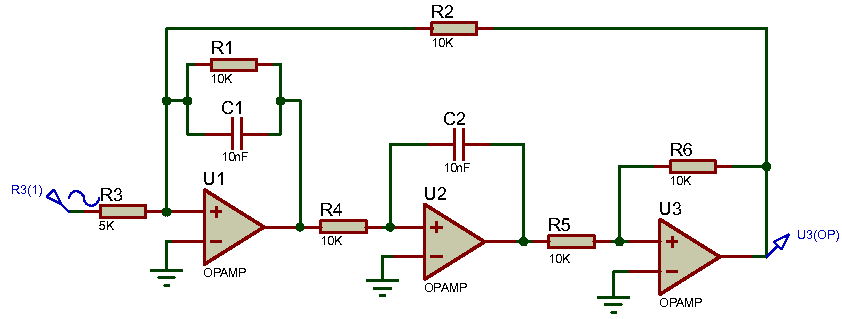
\includegraphics[width=\linewidth]{../Figures/a_ckt}
    \caption{Proteus circuit for Tow Thomas biquad circuit with output taken at $V_2$}
    \label{fig:protA}
\end{figure}
\proteusObservationA{protA}{6.02}{2.02}{lowpass filter designed in Problem 2}
\mysubsub{Bandpass Design}
\subproblem{Determine the nature of the response by observing output at $V_{O1}$ with input $V_1$.}
\begin{figure}[H]
    \centering
    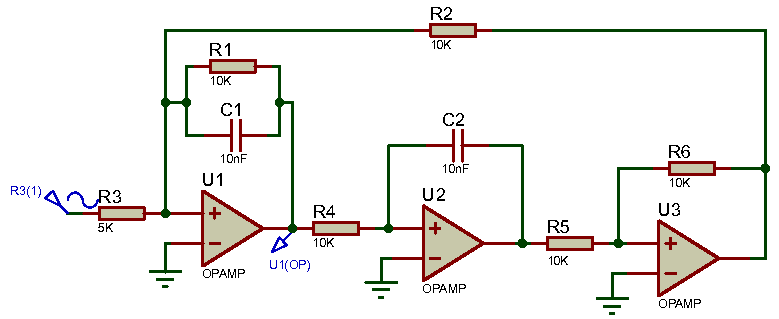
\includegraphics[width=\linewidth]{../Figures/b_ckt}
    \caption{Proteus circuit for Tow Thomas biquad circuit with output taken at $V_{O1}$}
    \label{fig:protB}
\end{figure}
\proteusObservationB{protB}{6.02}{1.58}{0.987, 2.58}{1.593}{bandpass filter designed in Problem 2}
\subproblem{Observe the magnitude response by obtaining each of the following filter from your design and note down passband gain and half power frequencies:}
\mysubsub{Highpass Design}
\subsubsection*{i. Highpass filter}
To design a highpass filter, we need a 4\textsuperscript{th} op-amp in addition to the 3 op-amp Tow Thomas biquad circuit. We first design a general circuit using the required filter parameters, and then choose values that constraint a highpass response. As derived earlier, the required condition for a highpass response at $V_2'$ is $R_1=R_2=R_3$.\\
The filter parameters for the required filter are, $\omega_o=10^4$, $Q=1$ and $H=1$ (for a highpass filter, $H=1$, as shown by comparing Equation~\ref{eqn:tfr_hp} and Equation~\ref{eqn:tfr_hp_final}).\\
We normalize the design at $\omega_o=1$ rad/s, $Q=1$ and $H=1$. Let us consider, $R_1=R_2=R_3=1\Omega$ and $C_2=1$ F. Using these values and the set of relations from Equation~\ref{eqn:relations} to calculate the remaining elemental values as,
 \begin{equation*}
    \begin{aligned}
       \omega_o^2&=\frac{1}{R_2R_4C_1C_2}\Rightarrow R_4C_1=1\\
       Q&=\sqrt{\frac{R_1^2C_1}{R_2R_4C_2}}\Rightarrow R_4=C_1
    \end{aligned}
\end{equation*}
Solving for $C_1$ and $R_4$, we get, $C_1=1$ F and  $R_4=1\Omega$.\\
Since the problem is to design the filter at $\omega_o=10^4$ rad/s, $K_f=10^4$. Let us choose $K_m=10^4$. Also, as the values of $R_5$ and $R_6$ don't affect in the actual response of the filter, we choose it as $R_5=R_6=1\Omega$. The scaled elemental values are,
 \begin{equation*}
    \begin{aligned}
       &R_1=1\times10^4=10 \text{ K}\Omega \quad &&R_2=1\times10^4=10 \text{ K}\Omega\\
       &R_3=0.5\times10^4=5 \text{ K}\Omega \quad &&R_4=1\times10^4=10 \text{ K}\Omega\\
       &R_5=1\times10^4=10 \text{ K}\Omega \quad &&R_6=1\times10^4=10 \text{ K}\Omega\\
       &C_1= \frac{1}{10^4\times10^4}=10\text{ nF} \quad && 
       C_2= \frac{1}{10^4\times10^4}=10\text{ nF}
    \end{aligned}
\end{equation*}
\textit{Note: The elemental notations are according to the Figure~\ref{fig:hp}.}
\begin{figure}[H]
    \centering
    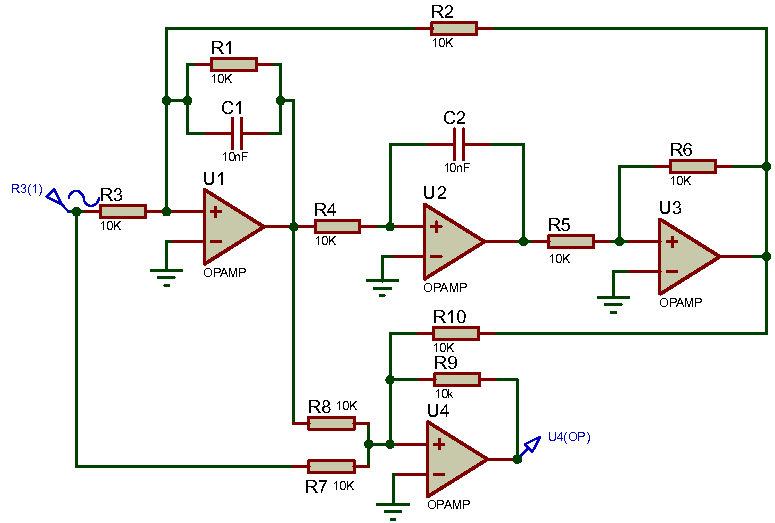
\includegraphics[width=\linewidth]{../Figures/c_ckt}
    \caption{Proteus circuit for highpass filter using 4-opamp biquad circuit}
    \label{fig:protC}
\end{figure}
\proteusObservationC{protC}{0}{1.25}{highpass filter designed in Problem 2}
\mysubsub{Bandstop Design}
\subsubsection*{ii. Bandstop filter}
To design a bandstop filter, we need a 4\textsuperscript{th} op-amp in addition to the 3 op-amp Tow Thomas biquad circuit. We first design a general circuit using the required filter parameters, and then choose values that constraint a bandstop response. As derived earlier, the required condition for a bandstop response at $V_2'$ is $R_1=R_3$.\\
The filter parameters for the required filter are, $\omega_o=10^4$, $Q=1$ and $H=2$.\\
We normalize the design at $\omega_o=1$ rad/s, $Q=1$ and $H=2$. Let us consider, $R_1=R_3=1\Omega$ and $C_2=1$ F. Using these values and the set of relations from Equation~\ref{eqn:relations} to calculate the remaining elemental values as,
\begin{equation*}
    \begin{aligned}
        H&=\frac{R_2}{R_3}\Rightarrow R_2=2\Omega\\
       \omega_o^2&=\frac{1}{R_2R_4C_1C_2}\Rightarrow R_4C_1=\frac{1}{2}\\
       Q&=\sqrt{\frac{R_1^2C_1}{R_2R_4C_2}}\Rightarrow 2R_4=C_1
    \end{aligned}
\end{equation*}
Solving for $C_1$ and $R_4$, we get, $C_1=1$ F and  $R_4=0.5\Omega$.\\
Since the problem is to design the filter at $\omega_o=10^4$ rad/s, $K_f=10^4$. Let us choose $K_m=10^4$. Also, as the values of $R_5$ and $R_6$ don't affect in the actual response of the filter, we choose it as $R_5=R_6=1\Omega$. The scaled elemental values are,
 \begin{equation*}
    \begin{aligned}
       &R_1=1\times10^4=10 \text{ K}\Omega \quad &&R_2=2\times10^4=20 \text{ K}\Omega\\
       &R_3=1\times10^4=10 \text{ K}\Omega \quad &&R_4=0.5\times10^4=5 \text{ K}\Omega\\
       &R_5=1\times10^4=10 \text{ K}\Omega \quad &&R_6=1\times10^4=10 \text{ K}\Omega\\
       &C_1= \frac{1}{10^4\times10^4}=10\text{ nF} \quad && 
       C_2= \frac{1}{10^4\times10^4}=10\text{ nF}
    \end{aligned}
\end{equation*}
\textit{Note: The elemental notations are according to the Figure~\ref{fig:bsap}.}
\begin{figure}[H]
    \centering
    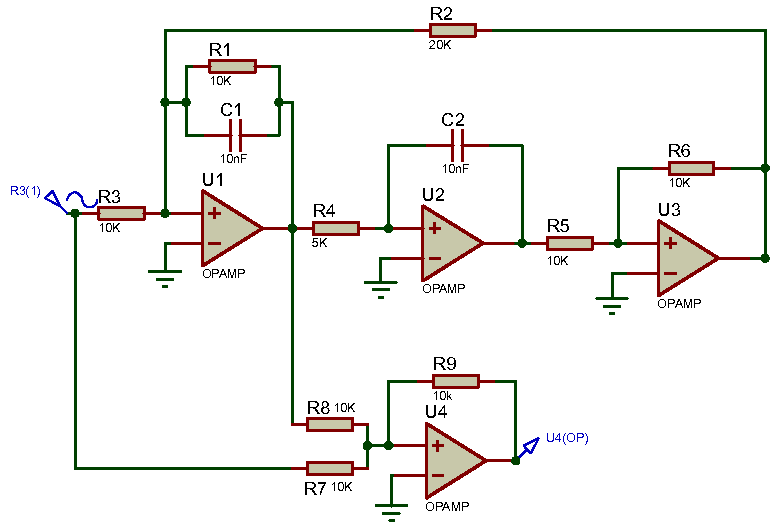
\includegraphics[width=\linewidth]{../Figures/d_ckt}
    \caption{Proteus circuit for bandstop filter using 4-opamp biquad circuit}
    \label{fig:protD}
\end{figure}
\proteusObservationB{protD}{0}{1.59}{0.978, 2.52}{1.642}{bandstop filter designed in Problem 2}
\mysubsub{Allpass Design}
\subsubsection*{ii. Allpass filter}
To design an allpass filter, we need a 4\textsuperscript{th} op-amp in addition to the 3 op-amp Tow Thomas biquad circuit. We first design a general circuit using the required filter parameters, and then choose values that constraint an allpass response. As derived earlier, the required condition for an allpass response at $V_2'$ is $R_3=\ddfrac{R_1}{2}$.\\
The filter parameters for the required filter are, $\omega_o=10^4$, $Q=1$ and $H=2$.\\
We normalize the design at $\omega_o=1$ rad/s, $Q=1$ and $H=2$. Let us consider, $R_1=1\Omega$, $R_3=0.5\Omega$ and $C_2=1$ F. Using these values and the set of relations from Equation~\ref{eqn:relations} to calculate the remaining elemental values as,
\begin{equation*}
    \begin{aligned}
        H&=\frac{R_2}{R_3}\Rightarrow R_2=1\Omega\\
       \omega_o^2&=\frac{1}{R_2R_4C_1C_2}\Rightarrow R_4C_1=1\\
       Q&=\sqrt{\frac{R_1^2C_1}{R_2R_4C_2}}\Rightarrow R_4=C_1
    \end{aligned}
\end{equation*}
Solving for $C_1$ and $R_4$, we get, $C_1=1$ F and  $R_4=1\Omega$.\\
Since the problem is to design the filter at $\omega_o=10^4$ rad/s, $K_f=10^4$. Let us choose $K_m=10^4$. Also, as the values of $R_5$ and $R_6$ don't affect in the actual response of the filter, we choose it as $R_5=R_6=1\Omega$. The scaled elemental values are,
 \begin{equation*}
    \begin{aligned}
       &R_1=1\times10^4=10 \text{ K}\Omega \quad &&R_2=1\times10^4=10 \text{ K}\Omega\\
       &R_3=0.5\times10^4=5 \text{ K}\Omega \quad &&R_4=1\times10^4=10 \text{ K}\Omega\\
       &R_5=1\times10^4=10 \text{ K}\Omega \quad &&R_6=1\times10^4=10 \text{ K}\Omega\\
       &C_1= \frac{1}{10^4\times10^4}=10\text{ nF} \quad && 
       C_2= \frac{1}{10^4\times10^4}=10\text{ nF}
    \end{aligned}
\end{equation*}
\textit{Note: The elemental notations are according to the Figure~\ref{fig:bsap}.}
\begin{figure}[H]
    \centering
    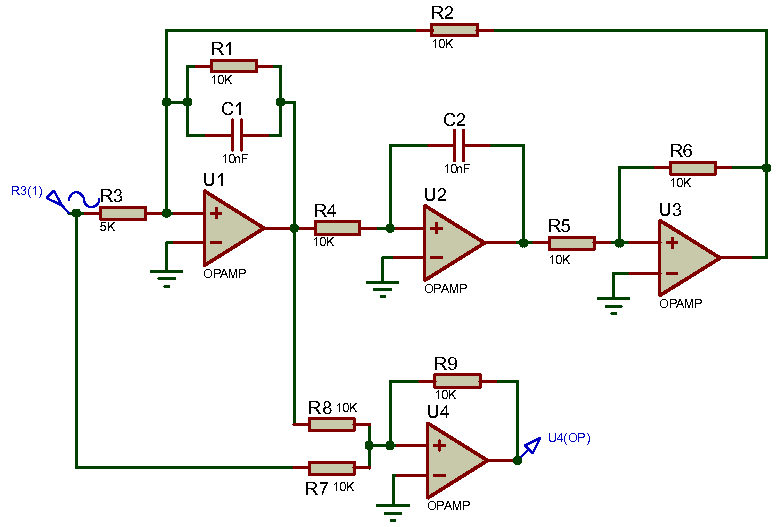
\includegraphics[width=\linewidth]{../Figures/e_ckt}
    \caption{Proteus circuit for allpass filter using 4-opamp biquad circuit}
    \label{fig:protE}
\end{figure}
\proteusObservationD{protE}{26.14}{allpass filter designed in Problem 2}

\mysub{Problem 3}
\problem{Realize the second order Butterworth lowpass filter having half power frequency of 3.5 KHz using the Tow Thomas biquad circuit and observe the response. By plotting the response show the half
power frequency and DC gain.}
For second order butterworth filter with half power frequency $\omega_o=1$ rad/s, the denominator function is,
\begin{equation*}
    \begin{aligned}
        f_{den}(s)&=s^2+\sqrt{2}s+1
    \end{aligned}
 \end{equation*}
 From Equation~\ref{eqn:tfr_lp}, the denominator function for a standard lowpass filter can be written as,
 \begin{equation*}
     f_{den}'(s)=s^2+s\left(\frac{\omega_o}{Q}\right)+\omega_o^2
 \end{equation*}
 Comparing these equations, we get,
 \begin{equation*}
     \begin{aligned}
         \omega_o^2=1&\Rightarrow\omega_o=\sqrt{1}=1\\
         \frac{\omega_o}{Q}=\sqrt{2}&\Rightarrow Q=\frac{\omega_o}{\sqrt{2}}=\frac{1}{\sqrt{2}}=0.7071
     \end{aligned}
 \end{equation*}
 The filter parameters for the required filter are, $\omega_o=3.5$ KHz, $Q=0.7071$ and $H=1$ (for a butterworth response, DC gain is unity).\\
We normalize the design at $\omega_o=1$ rad/s, $Q=0.7071$ and $H=1$. Let us consider, $R_4=1\Omega$, $C_1=C_2=1$ F. Using these values and the set of relations from Equation~\ref{eqn:relations} to calculate the remaining elemental values as,
\begin{equation*}
   \begin{aligned}
      \omega_o^2&=\frac{1}{R_2R_4C_1C_2}\Rightarrow R_2=1\Omega\\
      Q&=\sqrt{\frac{R_1^2C_1}{R_2R_4C_2}}\Rightarrow R_1=0.7071\Omega\\
      H&=\frac{R_2}{R_3}\Rightarrow R_3=1\Omega
   \end{aligned}
\end{equation*}
Since the problem is to design the filter at $\omega_o=3.5$ KHz, $K_f=\ddfrac{2\pi\times3.5\times10^3}{1}\approx22000$. Let us choose $K_m=10^4$. Also, as the value of $R_5$ doesn't affect in the actual response of the filter, we choose it as $R_5=1\Omega$. The scaled elemental values are,
 \begin{equation*}
    \begin{aligned}
       &R_1=0.7071\times10^4=7.071 \text{ K}\Omega \quad &&R_2=1\times10^4=10 \text{ K}\Omega\\
       &R_3=1\times10^4=10 \text{ K}\Omega \quad &&R_4=1\times10^4=10 \text{ K}\Omega\\
       &C_1= \frac{1}{22000\times10^4}=4.54\text{ nF} \quad && 
       C_2= \frac{1}{22000\times10^4}=4.54\text{ nF}\\
       &R_5=1\times10^4=10 \text{ K}\Omega
    \end{aligned}
\end{equation*}
\textit{Note: The elemental notations are according to the Figure~\ref{fig:ques}.}
\begin{figure}[H]
    \centering
    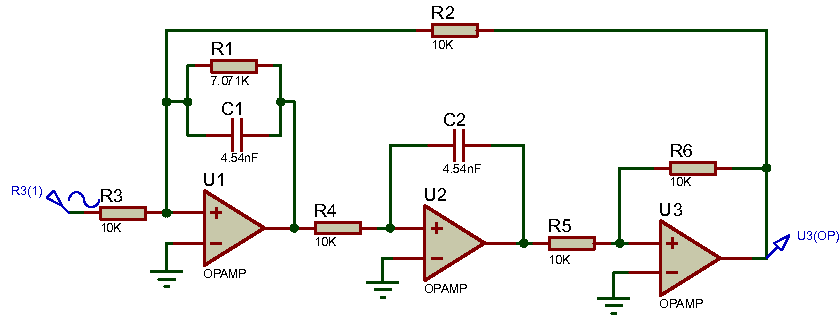
\includegraphics[width=\linewidth]{../Figures/f_ckt}
    \caption{Proteus circuit for lowpass filter using Tow Thomas biquad circuit}
    \label{fig:protF}
\end{figure}
\proteusObservationA{protF}{0}{3.49}{lowpass filter designed in Problem 3}
\section{Discussion and Conclusion}
In this lab experiment, we designed different types of filter using the Tow Thomas biquad circuit given in Figure~\ref{fig:ques}. The derivation for the different responses was understood as a part of the experiment. An important thing to note is that the single Tow Thomas biquad circuit gives lowpass response at $V_2$ and bandpass response at $V_{O1}$, which was also verified and visualized from the actual design problem. Similarly, to design highpass, bandstop and allpass filters, an additional op-amp was used along with the original Tow Thomas biquad circuit as shown in Figure~\ref{fig:bsap} and Figure~\ref{fig:hp}, with some constraints in the values of resistance such that response taken at $V_2'$ would be as we require. The design problems for these filters were also performed, and the observations are included above. Lastly, a second order butterworth filter was designed at half power frequency of $\omega_o=3.5$ KHz using the Tow Thomas biquad circuit. This was performed by comparing the transfer functions and then applying tuning algorithm to constraint the elemental values for the required filter parameters. \\
Hence, the objectives of the lab were fulfilled with the understanding of the mentioned topics.
\end{document}